\newpage
\begin{multicols}{2}
\chapter{Quick Start Guide}
	
Welcome to the quick start quide.  Following these steps, you will get your 
gain/phase analyser up and running in no time!

\end{multicols}
\begin{figure}[h]
\centering
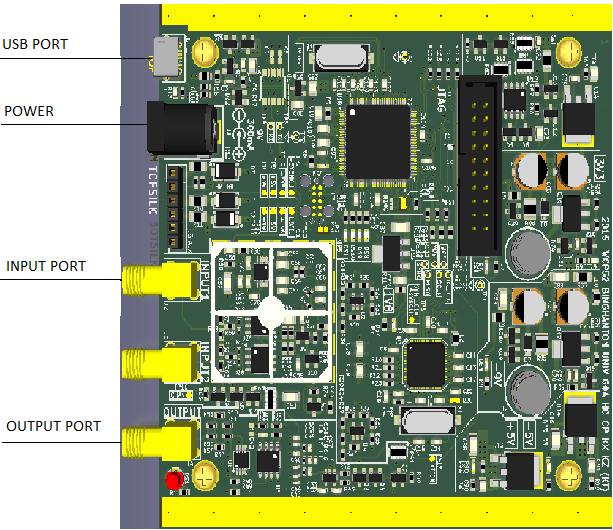
\includegraphics[width=6.5in]{getting_started/ports}
\caption{High level overview of gain/phase analyser}
\label{fig:highlevel}
\end{figure}

\begin{multicols}{2}
\section{Getting to know the device}

For the most basic use of the gain/phase analyser, you will be using the four ports described in the figure.
The USB Port is so that the device may connect to the computer.
Power is the port that you will plug the power supply into.  The board does not receive enough power from USB, so this is necessary for operation.
Input port receives signals from the filter that you are analysing.
Output port sends signals to the filter.


\section{Setting up your device}
\end{multicols}
\begin{center}
\missingfigure[figwidth=4in]{Photo}
\end{center}
\begin{multicols}{2}

First begin by connecting a filter to the board.  Connections for the filter must be made between the Output Port and Input Port.  The above figure shows us connecting a wire to the board.  You can do this as well just for learning purposes, but keep in mind that you will normally want to place a between these two ports.

\end{multicols}
\begin{center}
\missingfigure[figwidth=4in]{Photo}
\end{center}
\begin{multicols}{2}

Now, we will connect the device to a PC using a micro USB cable.  Place one side of the cable into the USB port and the other side into any USB port on your PC.

\end{multicols}
\begin{center}
\missingfigure[figwidth=4in]{Photo}
\end{center}
\begin{multicols}{2}

Now, we will provide power to the device.  Plug the power supply into the Power port as shown in the diagram.

Excellent job.  Now we move to the computer where we can take a measurement and get some results!  



